% APÉNDIZES

% Escribe cada apéndize como si fuera un capítulo más.

\chapter{Apéndice A: Más resultados experimentación SSLTree}
\label{resultados-experimentación}

Aquí se incluirán todos los resultados \textit{adicionales} que, por completitud, se desean incluir de la experimentación propuesta en \ref{metodologia}.

\section{Estudio del parámetro w}

\imagen{figuras/w_all_rankings_gini.png}{Mapa de calor de los rankings medios (Gini)}{Mapa de calor de los rankings medios (Gini).}{0.45}

Recurriendo de nuevo a un promedio es posible ver cuál es el ranking que ocupa cada valor de $w$:

\begin{table}[h]
\resizebox{\textwidth}{!}{%
\begin{tabular}{|c|c|c|c|c|c|c|c|c|c|c|}
\hline
\rowcolor[HTML]{FFCE93} 
{\color[HTML]{333333} 1} & {\color[HTML]{333333} \textbf{.9}} & {\color[HTML]{333333} .8} & {\color[HTML]{333333} .7} & {\color[HTML]{333333} .6} & {\color[HTML]{333333} .5} & {\color[HTML]{333333} .4} & {\color[HTML]{333333} .3} & {\color[HTML]{333333} .2} & {\color[HTML]{333333} .1} & {\color[HTML]{333333} 0} \\ \hline
5.12                     & \textbf{4.97}                      & 5.38                      & 5.49                      & 5.55                      & 5.88                      & 6.35                      & 6.26                      & 6.51                      & 6.98                       & 7.51                     \\ \hline
\end{tabular}%
}
\caption{Ranking promedio de cada valor de $w$ (Gini)}
\label{tab:ranking-w-gini}
\end{table}

La conclusión con Gini es la misma que para Entropy, el mejor valor de $w$ parece ser 0.9 en todos los datasets.

\section{Comparativa básica}

\imagen{figuras/comparativa_final_gini.png}{Ranking promedio de cada modelo para todos los datasets (Gini)}{Ranking promedio de cada modelo para todos los datasets (Gini).}{1}

Los resultados obtenidos indican que la implementación de SSLTree funciona correctamente y en general obtiene mejores resultados que el resto de modelos.

El análisis de diferencias críticas/significativas para el criterio Gini resulta en la misma conclusión. Aunque SSLTree sea mejor, no hay diferencias significativas que supongan una mejora grande.

\imagen{figuras/nemenyi_10_gini.png}{Comparativa básica: Nemenyi Test para 10\% de etiquetados (Gini)}{Comparativa básica: Nemenyi Test para 10\% de etiquetados (Gini).}{1}

\imagen{figuras/nemenyi_20_gini.png}{Comparativa básica: Nemenyi Test para 20\% de etiquetados (Gini)}{Comparativa básica: Nemenyi Test para 20\% de etiquetados (Gini).}{1}

\imagen{figuras/nemenyi_30_gini.png}{Comparativa básica: Nemenyi Test para 30\% de etiquetados (Gini)}{Comparativa básica: Nemenyi Test para 30\% de etiquetados (Gini).}{1}

\imagen{figuras/nemenyi_40_gini.png}{Comparativa básica: Nemenyi Test para 40\% de etiquetados (Gini)}{Comparativa básica: Nemenyi Test para 40\% de etiquetados (Gini).}{1}

\section{Comparativa entre ensembles}

\begin{mainbox}{Conjuntos de datos utilizados}
    Cierta función interna de la biblioteca \textit{SSLTree} utilizada en la comparación (Co-Forest) parece no soportar algún dato. Existe un conjunto de datos que, pese a construirse el árbol de decisión, arroja un error en ejecución. Para el criterio Gini, simplemente se ha ignorado este conjunto de datos. Las conclusiones no se han visto afectadas.
\end{mainbox}

\imagen{figuras/comparativa_ensembles_gini.png}{Ranking promedio de cada ensemble para todos los datasets (Gini)}{Ranking promedio de cada ensemble para todos los datasets (Gini).}{1}

Realizando un nuevo test de Nemenyi entre estos modelos, se observan prácticamente las mismas diferencias significativas en 10\% y 20\% de etiquetados que para \textit{entropy}. Estos resultados pueden verse en las figuras \ref{fig:figuras/nemenyi_10_ensembles_gini.png}, \ref{fig:figuras/nemenyi_20_ensembles_gini.png}, \ref{fig:figuras/nemenyi_30_ensembles_gini.png} y \ref{fig:figuras/nemenyi_40_ensembles_gini.png}.

\imagen{figuras/nemenyi_10_ensembles_gini.png}{Comparativa ensembles: Nemenyi Test para 10\% de etiquetados (Gini)}{Comparativa ensembles: Nemenyi Test para 10\% de etiquetados (Gini).}{1}

\imagen{figuras/nemenyi_20_ensembles_gini.png}{Comparativa ensembles: Nemenyi Test para 20\% de etiquetados (Gini)}{Comparativa ensembles: Nemenyi Test para 20\% de etiquetados (Gini).}{1}

\imagen{figuras/nemenyi_30_ensembles_gini.png}{Comparativa ensembles: Nemenyi Test para 30\% de etiquetados (Gini)}{Comparativa ensembles: Nemenyi Test para 30\% de etiquetados (Gini).}{1}

\imagen{figuras/nemenyi_40_ensembles_gini.png}{Comparativa ensembles: Nemenyi Test para 40\% de etiquetados (Gini)}{Comparativa ensembles: Nemenyi Test para 40\% de etiquetados (Gini).}{1}


\newpage
\chapter{Apéndice B: Visualizador GSSL}
\label{apendice-b}
En este anexo se comenta el desarrollo y resultado de una aplicación web sencilla diseñada a partir de los algoritmos desarrollados en la investigación. 

El objetivo es poder entender cómo funcionan los grafos, sus métodos de construcción y también cómo se propagan las etiquetas. Es accesible desde \url{https://dmacha.dev/gssl}.

\section{Motivación}

En la Universidad de Burgos se han realizado otras herramientas, tanto publicadas en revistas como proyectos de Trabajos de Fin de Grado (como \href{https://vass.dmacha.dev}{VASS}, realizada por el mismo autor que este trabajo), que están alineadas con la docencia de inteligencia artificial y \textit{machine learning}. De esta manera, se puede disponer de una nueva herramienta que pueda ser de ayuda para el aprendizaje de estudiantes, con aplicación concreta a los grafos en el aprendizaje semi-supervisado.

\section{Objetivos}

\begin{itemize}
    \item Modificar los algoritmos \Gls{gbili}, \Gls{rgcli} y \Gls{lgc} para la extracción de información de los pasos relevantes.
    \item Crear una \Gls{api} para la ejecución de los algoritmos y obtención de los pasos relevantes para su visualización Web.
    \item Crear la interfaz de usuario con la funcionalidad necesaria para la interpretación de la información.
\end{itemize}

\section{Tecnologías utilizadas}

Las tecnologías o herramientas utilizadas se enmarcan en dos grupos, por un lado, el \textit{frontend}, y por otro, el \textit{backend}.

En el \textit{frontend} se han utilizado varias bibliotecas destacables (todas gratuitas y libres) que han permitido generar las visualizaciones, estas son:

\begin{itemize}
    \item \textbf{Bootstrap}: Contiene código HTML, CSS y JavaScript que permite personalizar la interfaz del usuario actuando sobre los componentes mediante clases. Su objetivo es la creación de páginas web \textit{responsive} (adaptables). 
    \item     \textbf{jQuery}: Biblioteca muy utilizada que simplifica la programación de código JavaScript.
    \item \textbf{DataTables}: Permite crear tablas interactivas completamente personalizables con datos dinámicos.
    \item     \textbf{KaTeX}: Permite visualizar notación matemática en los navegadores y está basada en LaTeX.
    \item \textbf{Pseudocode}: Permite mostrar pseudocódigos de algoritmos tal y como se muestran en un documento generado por LaTeX. Utiliza KaTeX para renderizar fórmulas matemáticas.
    \item \textbf{D3.js}: Esta biblioteca es el núcleo de la aplicación. Permite generar, de forma automática, la visualización del grafo. Tiene un alto grado de libertad, lo que permite modificar completamente todos los aspectos del grafo (nodos, enlaces, colores, tamaños...).
    \item \textbf{introJS}: Esta biblioteca permite generar tutoriales interactivos en una página Web. En cada paso del tutorial, es posible seleccionar un elemento del la página junto com la explicación. El usuario puede navegar entre los pasos incluidos para comprender el funcionamiento.
\end{itemize}

Con respecto al \textit{backend}, está implementado en Python y además de los propios algoritmos investigados y alguna utilidad creada para este proyecto, se han utilizado varias bibliotecas conocidas en \textit{machine learning} y utilizadas en el resto de la maestría:

\begin{itemize}
    \item \textbf{pandas}: Biblioteca muy utilizada sobre manipulación de datos que define nuevas estructuras de datos capaces de realizar operaciones de interés de manera eficiente.
    \item \textbf{scikit-learn}: Es la biblioteca más utilizada en \textit{machine learning} en Python, incluye numerosos algoritmos de aprendizaje así como multitud de utilidades de procesamiento.
    \item \textbf{numpy}: Biblioteca dedicada al cálculo científico, implementa estructuras de datos tipo \textit{arrays} y matrices y funciones matemáticas para realizar operaciones de forma eficiente (de hecho, buena parte de su implementación está codificada en lenguaje C).
    \item \textbf{scipy}:  Biblioteca de algoritmos matemáticos.
    \item \textbf{flask}: Es un \textit{framework} en Python para desarrollar aplicaciones web. Es el núcleo de toda la aplicación.
\end{itemize}

\section{Desarrollo}
En esta sección se describen todas las decisiones de diseño y desarrollo que se han realizado para cumplir los objetivos.

\begin{mainbox}{Código de la implementación}
    La implementación completa de la web puede encontrarse en \url{https://github.com/dmacha27/TFM-VIU/tree/main/web}. 
\end{mainbox}

\subsection{Diseño arquitectónico}
La aplicación posee una arquitectura de dos capas. Esto es así porque como se quería desarrollar una aplicación sencilla, no se ha utilizado una tercera capa de datos (bases de datos) que suele ser común y que se catalogaría como arquitectura de tres capas.\\

\noindent\textbf{\large Arquitectura de dos capas} \\
Esta arquitectura esta formada por dos capas: capa de presentación y capa de aplicación (también conocida como capa o ``lógica de negocio''). En la figura \ref{fig:figuras/arq.png} se representa un diagrama con esta arquitectura.

\imagen{figuras/arq.png}{Arquitectura de dos capas}{Arquitectura de dos capas.}{0.5}

\begin{itemize}
    \item \textbf{Capa de presentación}: permite al usuario interactuar con el sistema. Se encarga de mostrar, y en este caso visualizar, la información que la aplicación desea. El contenido de esta capa es ejecutado en el propio navegador del usuario. El \textit{framework} Flask comentado anteriormente es el encargado de generar, para el usuario, todo el conjunto de plantillas, estilos y código dinámico (JavaScript) que el navegador ejecuta. De forma práctica, Flask es la capa de presentación.
    \item \textbf{Capa de aplicación}: maneja las peticiones de la capa de presentación y envía las respuestas apropiadas. También conocida como lógica de negocio, recibe este nombre porque es aquí donde está definida toda la funcionalidad de la aplicación. Esta capa está implementada en Python y es todo el código que se ejecuta en las rutas de la API definida. En este caso, por ejemplo, sería la ejecución de un algoritmo concreto.
\end{itemize}

La comunicación entre estas capas se realiza mediante el protocolo HTTPS (Protocolo de Transferencia de Hipertexto Seguro).


\subsection{Diseño procedimental}

En esta sección se describe la interacción del usuario con el sistema para visualizar un algoritmo. Los pasos que el usuario realiza son los siguientes (queda reflejado en la figura \ref{fig:sec}):

\begin{enumerate}
    \item El usuario accede a la web mediante su navegador y el servidor generará la plantilla HTML (y estilado) principal (carga del conjunto de datos).
    \item El usuario carga un conjunto de datos que será almacenado en el propio navegador. También se solicita al servidor la información básica de los datos (nombre de las columnas). El navegador permitirá pasar al apartado de configuración.
    \item El usuario configura su ejecución seleccionando los parámetros generales (como el nombre del atributo de la clase) y los específicos de cada algoritmo.
    \item El navegador realizará una petición al servidor con esa configuración a la espera de una respuesta con toda la información de la ejecución.
    \item El servidor entonces carga de forma dinámica el conjunto de datos, ejecuta el algoritmo de construcción de grafos y ejecuta el algoritmo de inferencia de etiquetas. El servidor recopila y procesa la información de los pasos realizados y construye la respuesta (JSON).
    \item EL navegador procesa la información y genera las visualizaciones correspondientes para el usuario.
\end{enumerate}

\begin{figure}[H]
		\centering
		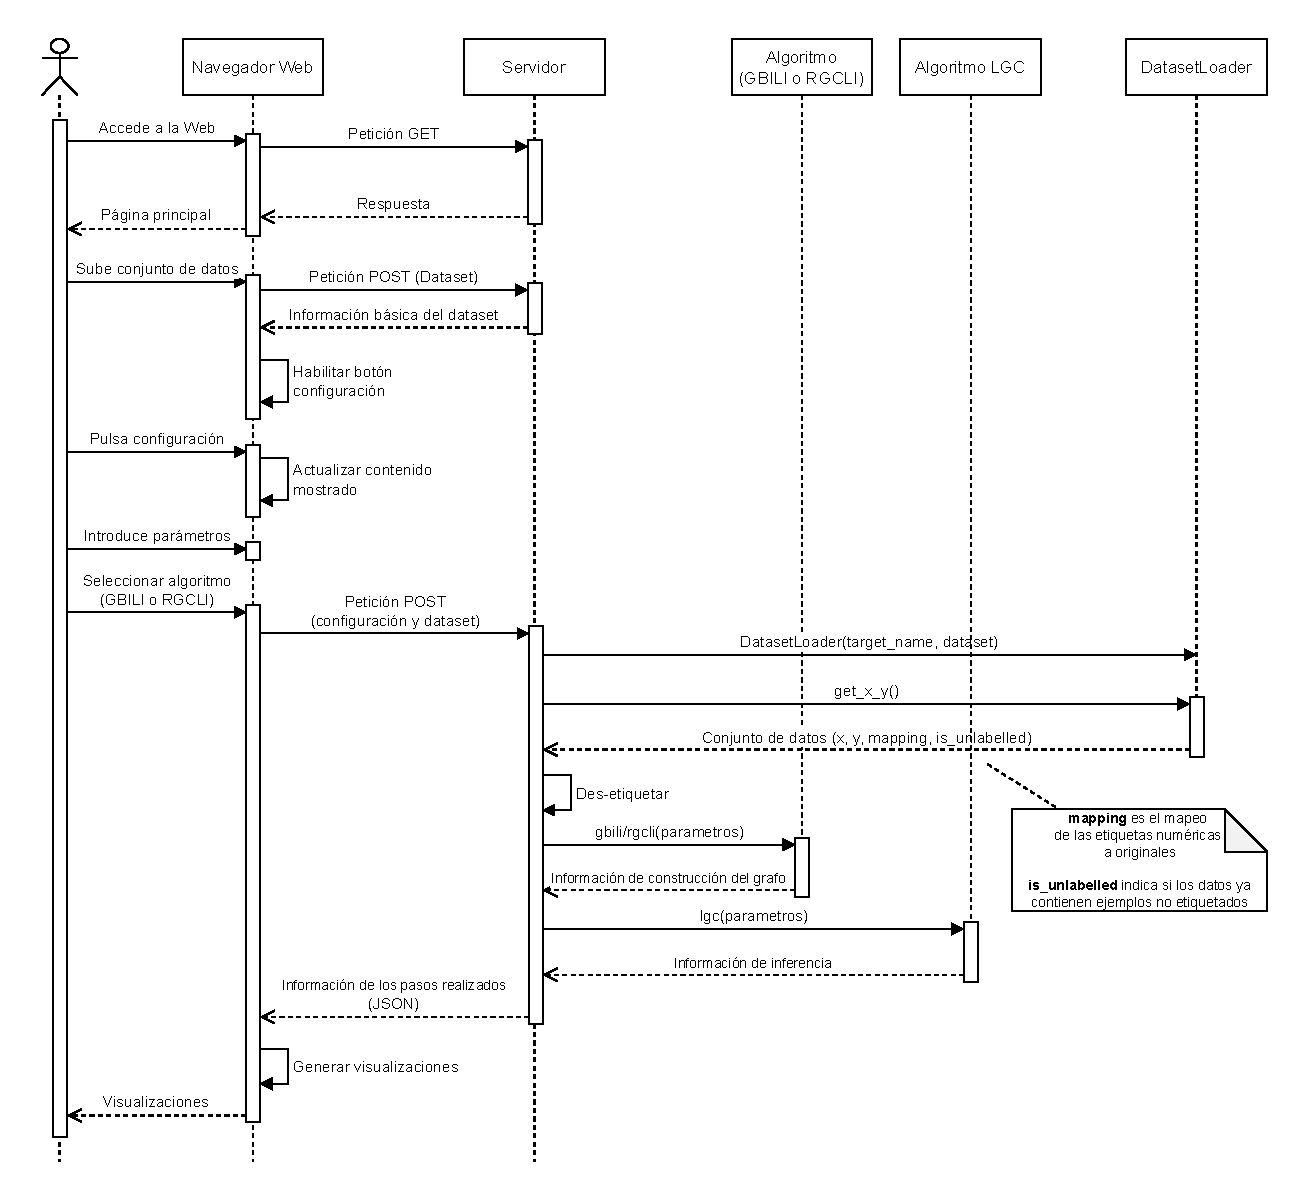
\includegraphics[width=1\textwidth]{figuras/sec.pdf}
		\caption[Diagrama de secuencia]{\textbf{Diagrama de secuencia.}}\label{fig:sec}
\end{figure}

\subsection{Diseño de datos}

En esta sección se describe la información que fluye entre el servidor y el cliente. La figura \ref{fig:sec} representa esa última respuesta del servidor (``Información de los pasos realizados'').

El diseño de la lógica está pensado de tal forma que dependiendo qué algoritmo de construcción de grafo se quiera visualizar, se realiza una petición a una ruta u otra. Esto quiere decir que, salvo la información de los pasos de la construcción (GBILI o RGCLI), el resto es común (el algoritmo de inferencia LGC). El objetivo de ambas rutas es responder con un texto tipo \Gls{json}, que JavaScript es capaz de manejar de forma nativa y directa.


\lstset{
    language=Python,
    basicstyle=\ttfamily\small,
    keywordstyle=\color{blue},
    stringstyle=\color{red},
    commentstyle=\color{green},
    backgroundcolor=\color{white},,
    breaklines=true,
    breakatwhitespace=false,
    showspaces=false,
    showstringspaces=false,
    showtabs=false,
    tabsize=4,
    captionpos=b
}


El aspecto de una respuesta de las rutas es algo parecido a la figura \ref{fig:response}. Siempre existe una entrada que representa los pasos del algoritmo de construcción y otra para el algoritmo de inferencia. Sigue una estructura típica de diccionario con claves y valores. La estructura se organiza por niveles. En el primer nivel se hace referencia al algoritmo, en el segundo se hace referencia a cada paso dentro de un algoritmo y en el tercer nivel se encuentra la información interesante del paso.
En este último caso, es de destacar que siempre se informa de los nodos (los ejemplos en el conjunto de datos), de los enlaces que unen dichos nodos de cada paso (los enlaces de un paso pueden no ser los mismo que otro) e información adicional interesante del paso.

\begin{figure}[H]
    \centering
    \begin{minipage}{0.9\linewidth}
        \begin{center}
            \begin{lstlisting}
                    response = {
                    
                        "gbili": {
                            "PASO X": {
                                "nodes": nodes,
                                "links": link_list,
                                "+INFO": INFO
                            }
                        },
                    
                        "lgc": {
                            "PASO X": {
                                "nodes": nodes,
                                "links": link_list,
                                "+INFO": INFO
                            }
                        }
                    }
                    
                    return jsonify(response)
            \end{lstlisting}
        \end{center}
    \end{minipage}
    \caption{Estructura de la respuesta}
    \label{fig:response}
\end{figure}


\noindent\textbf{\large Pasos de GBILI} \\
Los pasos más relevantes que se han querido mostrar son: construcción de la matriz de distancias, obtención de los vecinos más cercanos, obtención de los vecinos mutuos, conectar vecinos cercanos a puntos etiquetados y el grafo final. Todo estos pasos están descritos en \ref{teoria-gbili} y mostrados en el pseudocódigo \ref{gbili}.

\begin{figure}[h!]
    \centering
    \begin{minipage}{0.9\linewidth}
        \begin{center}
            \begin{lstlisting}
                "gbili": {
                    "dataset": {
                        "nodes": nodes,
                        "links": [],
                        "distance": D.tolist()
                    },
                    "knn": {
                        "nodes": nodes,
                        "links": links_knn,
                        "neighbors": D_argsort.tolist()
                    },
                    "m_knn": {
                        "nodes": nodes,
                        "links": links_m_knn,
                        "mneighbors": m_knn
                    },
                    "semi_graph": {
                        "nodes": nodes,
                        "links": links_semi_graph,
                        "components": [component_membership_semi[i] for i in range(len(X))],
                        "components_with_labeled": list(components_with_labeled)
                    },
                    "graph": {
                        "nodes": nodes,
                        "links": links_graph,
                        "unions": list(unions),
                        "components": [component_membership_graph[i] for i in range(len(X))]
        
                    }
                }
            \end{lstlisting}
        \end{center}
    \end{minipage}
    \caption{Pasos GBILI}
    \label{fig:pasos-gbili}
\end{figure}

\begin{enumerate}
    \item \textit{\textbf{dataset}}: En este paso no existen enlaces todavía, se incluye la matriz de distancias D de cada par de nodos.
    \item \textit{\textbf{knn}}: En este paso, los enlaces representan uniones entre los vecinos más cercanos. Un elemento de la lista de enlaces tiene la forma:\\
    \begin{minipage}{\linewidth}
        \begin{center}
            \begin{lstlisting}
                    {"source": nodo origen, 
                    "target": nodo destino, 
                    "value": fuerza del enlace}
            \end{lstlisting}
        \end{center}
    \end{minipage}
    
    Además, se incluyen esos vecinos más cercanos de cada nodo como una lista (la posición i-ésima contiene los vecinos más cercanos del nodo i). 
    \item \textit{\textbf{m\_knn}}: En este paso, los enlaces representan uniones entre los vecinos más cercanos mutuos. Además, se incluyen esos vecinos más cercanos mutuos de cada nodo como una lista (la posición i-ésima contiene los vecinos más cercanos mutuos del nodo i).
     \item \textit{\textbf{semi\_graph}}: En este paso, los enlaces creados son parte del grafo final. Se incluye también un listado que indica la componente a la que pertenece cada nodo (la posición i-ésima contiene el número de componente a la que pertenece el nodo i). Por último, se construye un listado con las componentes que tienen algún punto etiquetado en ellas.
     \item \textit{\textbf{graph}}: Los enlaces representan el grafo final construido. ``unions'' es una lista de tuplas de dos elementos en la que cada una contiene el número de las dos componentes unidas. Se incluye de nuevo un listado que indica la componente a la que pertenece cada nodo (en el grafo final).
\end{enumerate}

\newpage
\noindent\textbf{\large Información de RGCLI} \\
Para RGCLI, los pasos más relevantes que se han querido mostrar son: construcción de la matriz de distancias, obtención de los vecinos más cercanos, el más cercano etiquetado y el k-ésimo más lejano y, por último, el grafo final construido. Todo estos pasos están descritos en \ref{teoria-rgcli} y mostrados en el pseudocódigo \ref{rgcli}.

\begin{figure}[h!]
    \centering
    \begin{minipage}{0.9\linewidth}
        \begin{center}
            \begin{lstlisting}
                "rgcli": {
                    "dataset": {
                        "nodes": nodes,
                        "links": [],
                        "distance": D.tolist()
                    },
                    "searchknn": {
                        "nodes": nodes,
                        "links": links_knn,
                        "kNN": kNN.tolist(),
                        "L": L.tolist(),
                        "F": F_rgcli.tolist()
                    },
                    "graph": {
                        "nodes": nodes,
                        "links": links_graph
                    }
                }
            \end{lstlisting}
        \end{center}
    \end{minipage}
    \caption{Pasos RGCLI}
    \label{fig:pasos-rgcli}
\end{figure}

\begin{enumerate}
    \item \textit{\textbf{dataset}}: En este paso no existen enlaces todavía, se incluye la matriz de distancias D de cada par de nodos.
    \item \textit{\textbf{searchknn}}: En este paso, los enlaces representan uniones entre los vecinos más cercanos. El formato de la lista de enlaces es el mismo que para GBILI. Además, se incluyen esos vecinos más cercanos mutuos de cada nodo del mismo modo que en GBILI, el etiquetado más cercano de cada nodo y el k-ésimo más lejano.
     \item \textit{\textbf{graph}}: Los enlaces representan el grafo final construido.
\end{enumerate}

\noindent\textbf{\large Información de \Gls{lgc}} \\
Este algoritmo es común para los dos anteriores y los pasos más relevantes que se han querido mostrar son: construcción de afinidad, creación de la matriz S, el proceso iterativo de inferencia y, por último, el etiquetado de los datos. Todo estos pasos están descritos en \ref{teoria-lgc} y mostrados en el pseudocódigo \ref{lgc}.

\begin{figure}[h!]
    \centering
    \begin{minipage}{0.9\linewidth}
        \begin{center}
            \begin{lstlisting}
                "lgc": {
                    "affinity": {
                        "nodes": nodes,
                        "links": links_graph,
                        "F": F.tolist(),
                        "W": W.tolist(),
                    },
                    "S": {
                        "nodes": nodes,
                        "links": links_graph,
                        "D": D_diag.tolist(),
                        "D_sqrt_inv": D_sqrt_inv.tolist(),
                        "S": S.tolist(),
                    },
                    "iteration": {
                        "nodes": nodes,
                        "links": links_graph,
                        "F_history": F_t_history.tolist(),
                        "pred_history": pred_history.tolist()
                    },
                    "labels": {
                        "nodes": nodes_final,
                        "links": links_graph,
                        "F_final": F_t_history[-1].tolist(),
                        "pred_final": pred_history[-1].tolist()
                    }
                }
            \end{lstlisting}
        \end{center}
    \end{minipage}
    \caption{Pasos LGC}
    \label{fig:pasos-lgc}
\end{figure}

Algo común a todos los pasos es que los enlaces representan el grafo final construido (proveniente de unos de los algoritmos anteriores). La demás información se resume en:
\begin{enumerate}
    \item \textit{\textbf{dataset}}: Se incluye la matriz de afinidad (W) y también una matriz de etiquetado similar a \ref{matriz-etiquetado} (F), que representa las etiquetas de cada nodo.
    \item \textit{\textbf{S}}: En este paso se calcula la matriz S (versión normalizada de W). Para su cálculo se utiliza $D$ y $D^{-1/2}$. Se incluyen ambas matrices y la matriz $S$. En realidad, su inclusión solo es por completitud, es interesante ver el formato de esa nueva matriz $D$ (que es diagonal).
    \item \textit{\textbf{iteration}}: Incluye un historial tanto de las etiquetas de cada nodo ``pred\_history'' (una lista de listas de una dimensión) como de la matriz de etiquetado ``F\_history'' (una lista de matrices donde cada una es como \ref{matriz-etiquetado} y se tiene una por cada iteración de LGC).
    \item \textit{\textbf{labels}}: Incluye la última lista de ``pred\_history'' (``pred\_final'') y la última matriz de etiquetado ``F\_final'' (``F\_final'').
\end{enumerate}